\documentclass{article}
\usepackage[utf8]{inputenc}
\usepackage[a4paper,hmargin=1.2in,vmargin=1.5in]{geometry}
\usepackage[parfill]{parskip}
\usepackage{hyperref}
\usepackage{enumitem}
\usepackage{amsmath}
\usepackage{amsthm}
\usepackage{amssymb}
\usepackage{listings}
\usepackage{xcolor}
\usepackage{floatrow}
\usepackage{graphicx}
\bibliographystyle{plainurl}
\usepackage{caption}
\usepackage{fancyhdr}
\usepackage{listings}

\renewcommand{\footrulewidth }{1 pt}
\pagestyle{fancy}
\fancyhf{}
\fancyhead[R]{Software Systems Laboratory}
\fancyhead[L]{20005002-200050147}
\cfoot{Page \thepage}

\newcounter{main}
\setcounter{main}{1}

\lstnewenvironment{code}[1][firstnumber=\themain,name=main]
  {
  \refstepcounter{main}
  \label{env: listing}
  \begin{center}
    \textbf{\large{Listing 1: [LaTeX]TeX}} \\
    % \textbf{Algorithm Boilerplate}
    \textbf{Packages imported in the original}
  \end{center}
  \lstset{
           language=[LaTeX]TeX,
           backgroundcolor=\color{white},   
           commentstyle=\color{green!30!black},
           stringstyle=\color{violet},
           keywordstyle=\color{blue}\bfseries,
           numbers=left,
           numberstyle=\tiny\color{gray},
          }
}
{\setcounter{main}{\value{lstnumber}}}

\usepackage[ruled,linesnumbered]{algorithm2e}
\RestyleAlgo{ruled}
\SetArgSty{textnormal}

\usepackage[square,numbers]{natbib}
\hypersetup{
    linkbordercolor=red,
    urlbordercolor=cyan
}

\theoremstyle{definition}
\newtheorem{definition}{Definition}[section]
\begin{document}

\section{Basic Theory of Linear Recurrences}

We all know about the Fibonacci Sequence, given by the recurrence
$$ f_{n+2} = f_{n+1} + f_{n}$$
and initialised as $f_0 = 0, f_1 = 1$. This is an instance of what is called a Linear Recurrence Sequence, or LRS.

\begin{definition}
\label{LRS}
\emph{LRS $(u_n)_{n=0}^{\infty}$ of order $k$ over field $\mathbb{F} $ is the sequence determined by the recurrence}
\begin{equation}
    u_{n+k} = \sum_{j=0}^{k-1} a_j u_{n+j}
\label{eq:fibonacci sequence}
\end{equation} 
\emph{for integers $n \geq 0$ with $a_0,\dots ,a_{k-1} \in \mathbb{F}$, $a_0 \neq 0$, and an initialization vector}

$$ [u_0\hspace{2mm}\dots \hspace{2mm}u_{k-1}]^T \in \mathbb{F}^{k\times1} $$

Thanks to Definition $\ref{LRS}$, when we say that we are given $(u_n)_{n=0}^{\infty}$ of order $k$ over $\mathbb{F}$, we actually
mean that we are given the $2k$ constants $a_0,\dots a_{k-1},u_0,\dots ,u_{k-1} \in \mathbb{F}$.
\end{definition}

The Fibonacci sequence shows up a lot in pop culture and DSA assignments, however, the study of LRS is a vast subject in its own right, with applications in software verification, quantum computing, formal languages, statistical physics, combinatorics, and theoretical biology, to name a few.

\subsection{Computing terms of an LRS}

For a fixed $k$, assuming we can do arithmetic operations in $\mathbb{F}$ in constant time, how long does it take to compute the $n^{th}$ term of a given LRS?

\begin{algorithm}
\caption{Naive first attempt naive}\label{alg:one}
\KwData{LRS $(u_n)_{n=0}^{\infty}$, n}
\KwResult{$u_n$}
\BlankLine
\If{$n < k$}{
\Return $u_n$
}
\Return $\sum_{j=0}^{k-1}a_j \cdot \mathsf{naive} \hspace{1mm} ((u_n)_{n=0}^{\infty},n-k+j)$
\end{algorithm}

% doubt in " " symbol of naive
By the way, notice the use of \verb|\mathsf| to write $\mathsf{"naive"}$. This algorithm,
unfortunately, is painfully inefficient: as you can see, the number of recursive calls will be exponentially many in $n$. This immediately prompts a more
“bottom-up”\footnote{Not to be confused with the drinking phrase} approach: we start from
the first $k$ terms, use them to compute the next term, and iterate this way upto $n$.
This takes $\mathcal{O}(n)$ iterations\footnote{In complexity analysis, the base of the
logarithm is implicitly taken as 2}.

But we can do better, in fact, we only need $\mathcal{O}(n \log {}n)$ iterations.

Technically, even Algorithm 2 is \textit{inefficient}: when we analyse complexity, we do it with respect to the size of the \textit{bit representation} of the input, i.e. how many bits it takes to
specify the input. An integer n takes log n bits to represent, so the parameter for
describing complexity is not $n$, but $\eta = $ log $n$.

%add the rest part%
\begin{algorithm}[ht]

\caption{Bottom up dynamic programming approach bottomup}

\KwData{LRS $(u_n)_{n=0}^{\infty}$, n}  
\KwResult{$u_n$}
\If{$n<k$}{
\Return $u_n$ \\
}
circularArray $\gets \{u_0,\dots u_{k-1}\}$\\
arrayStartIndex $\gets0$\\
$n_{last}\gets k-1$\\
\While{$n_{last}<n$}{
 nextTerm $\gets \sum_{j=0}^{k-1} \cdot $ circularArray[(arrayStartIndex+j)\%j] \\
 circularArray[arrayStartIndex] $\gets$ nextTerm\\
 arrayStartIndex $\gets$ (arrayStartIndex + 1)\%k \\
 $n_{last} \gets n_{last} + 1$ \\ 
}
\Return circularArray[(arrayStartIndex + k - 1)\%k]
\end{algorithm}

Yes, we can compute the $n^{th}$ term with $\mathcal{O}(\eta)$ operations, and the trick
here is a method called \textbf{iterated squaring}. Given an LRS $(u_n)_{n=0}^{\infty}$,
define its companion matrix \textbf{M} $\in \mathsf{F}^{k\times k}$ as

\begin{equation}
\label{eq: iterated squaring}
    \textbf{M} = 
    \begin{bmatrix}
        0 & 1 & 0 & \cdots & 0 \\
        0 & 0 & 1 & \cdots & 0 \\
        \vdots & \vdots & \vdots & \ddots & 1 \\
        0 & 0 & 0 & \cdots & 1 \\
        a_{0} & a_{1} & a_{2} & \cdots & a_{k-1} \\
    \end{bmatrix}
\end{equation}

Compare equations \ref{eq:fibonacci sequence} and \ref{eq: iterated squaring} and observe that
\begin{equation}
    \textbf{M}^n
    \begin{bmatrix}
        u_0 \\
        \vdots \\
        u_{k-1} \\
    \end{bmatrix}
    =
    \begin{bmatrix}
        u_n \\
        \vdots \\
        u_{n+k-1} \\
    \end{bmatrix}
\end{equation}

Iterated squaring hinges on this ridiculously trivial observation: consider the (unique!) binary representation of $n$: if you append a 0 to it, it becomes $2n$, if you append a 1, it becomes $2n + 1$.

Given \textbf{M}, to compute $\textbf{M}^n$, all we have to do is start with \textbf{I}, read the binary representation of $n$ from most to least significant: if at some point we have $\textbf{M}^i$, $\textbf{M}^j \cdot \textbf{M}^j = \textbf{M}^{2j}$, $\textbf{M}^{2j} \cdot \textbf{M} = \textbf{M}^{2j+1}$

In Algorithm \ref{alg:three}, we use a data structure called a \textbf{stack}. The constant time operations it supports are
\begin{itemize}
  \item pushing an element onto the top of the stack
  \item popping an element from the top of the stack (i.e. deleting the topmost element)
  \item reading the topmost element
  \item checking whether the stack is empty
\end{itemize}
 
As you can see, it's Last In, First Out.

The division while loop gets the bits of n from least to most significant, the iterated square while loop uses the bits from most to least significant. A stack fits the bill.

\begin{algorithm}

\caption{Iterated squaring approach efficient}\label{alg:three}

\KwData{LRS $(u_n)_{n=0}^{\infty}$, n}
\KwResult{$u_n$}
     quotient $\ \gets\ n $\\
     operationStack $\ \gets\ \{\} $\\
     \textbf{M}$\ \gets\ $companion($(u_n)_{n=0}^{\infty}$)  \\
     \textbf{x}$\ \gets $ $[u_0 \dots u_{k-1}]^\top $  \\
     \textbf{A}$\ \gets \textbf{I}_{k\times k}$ \\
\While{ $\text{quotient} \neq 0$}{
    push(operationStack, quotient\%2) \\
    quotient\ $\gets $ quotient/2 \\
}
\While{ $\text{operationStack} \neq \{\} $}{
    $\textbf{A}\ \gets \textbf{A} \cdot \textbf{A}$  \\
    \If{\text{top(operationStack)} = 1}{
       $ \textbf{A}\ \gets\ \textbf{A} \cdot \textbf{M}$ 
    }
    pop(operationStack) 
}
 $\textbf{y} \ \gets  \textbf{Ax} $\\
\Return \textbf{y}[0]

\end{algorithm}



\subsection{Problems associated with LRS}
Surprisingly, the following rather simple \textit{decision problem}\footnote{Given
an arbitrary input, answer a particular question about it with Yes or No},referred to as the Skolem problem,has been open for the last eight decades or so.

\begin{definition}[Skolem problem]
\emph{For the arbitrary LRS $(u_n)_{n=0}^{\infty}$ whose description is given as input, does there exist an integer $n \geq 0$ such that $u_n = 0$?}
\end{definition}

This has a bunch of equivalent formulations, and by being open, we mean that nobody really knows of an algorithm that can decide it (the algorithm should terminate and give the correct answer for $all$ possible inputs), or whether there is such an algorithm at all.

We can also consider another related problem for LRS over fields where the $>$ operator is defined:

\begin{definition}[Positivity problem]
\emph{For the arbitrary LRS $(u_n)_{n=0}^{\infty}$ whose description is given as input, does there exist an integer $n \geq 0$ such that $u_n = 0$?}
\end{definition}

Deciding even special cases of these problems (i.e. restricting what kind of LRS can be fed as input) requires sophisticated maths, like Kronecker’s theorem on Diophantine approximations,\cite[][Chap. 7, Sec. 1.3, Prop. 7]{bourbaki1966general}, and profound properties of “algebraic” numbers \cite{mignotte1982some} and then some more mathematical arsenal \cite{bell2007positivity,renegar1992computational}

If you found this short write up interesting, \href{https://fmindia.cmi.ac.in/update2013/presentations/S-Akshay.pdf}{here} is a survey talk about the problem, given not so long ago.

\section{Programming}

\subsection{Screenshot}
\begin{figure}[H]
        \CommonHeightRow{
            \begin{floatrow}[2]
                \ffigbox[\FBwidth]
                {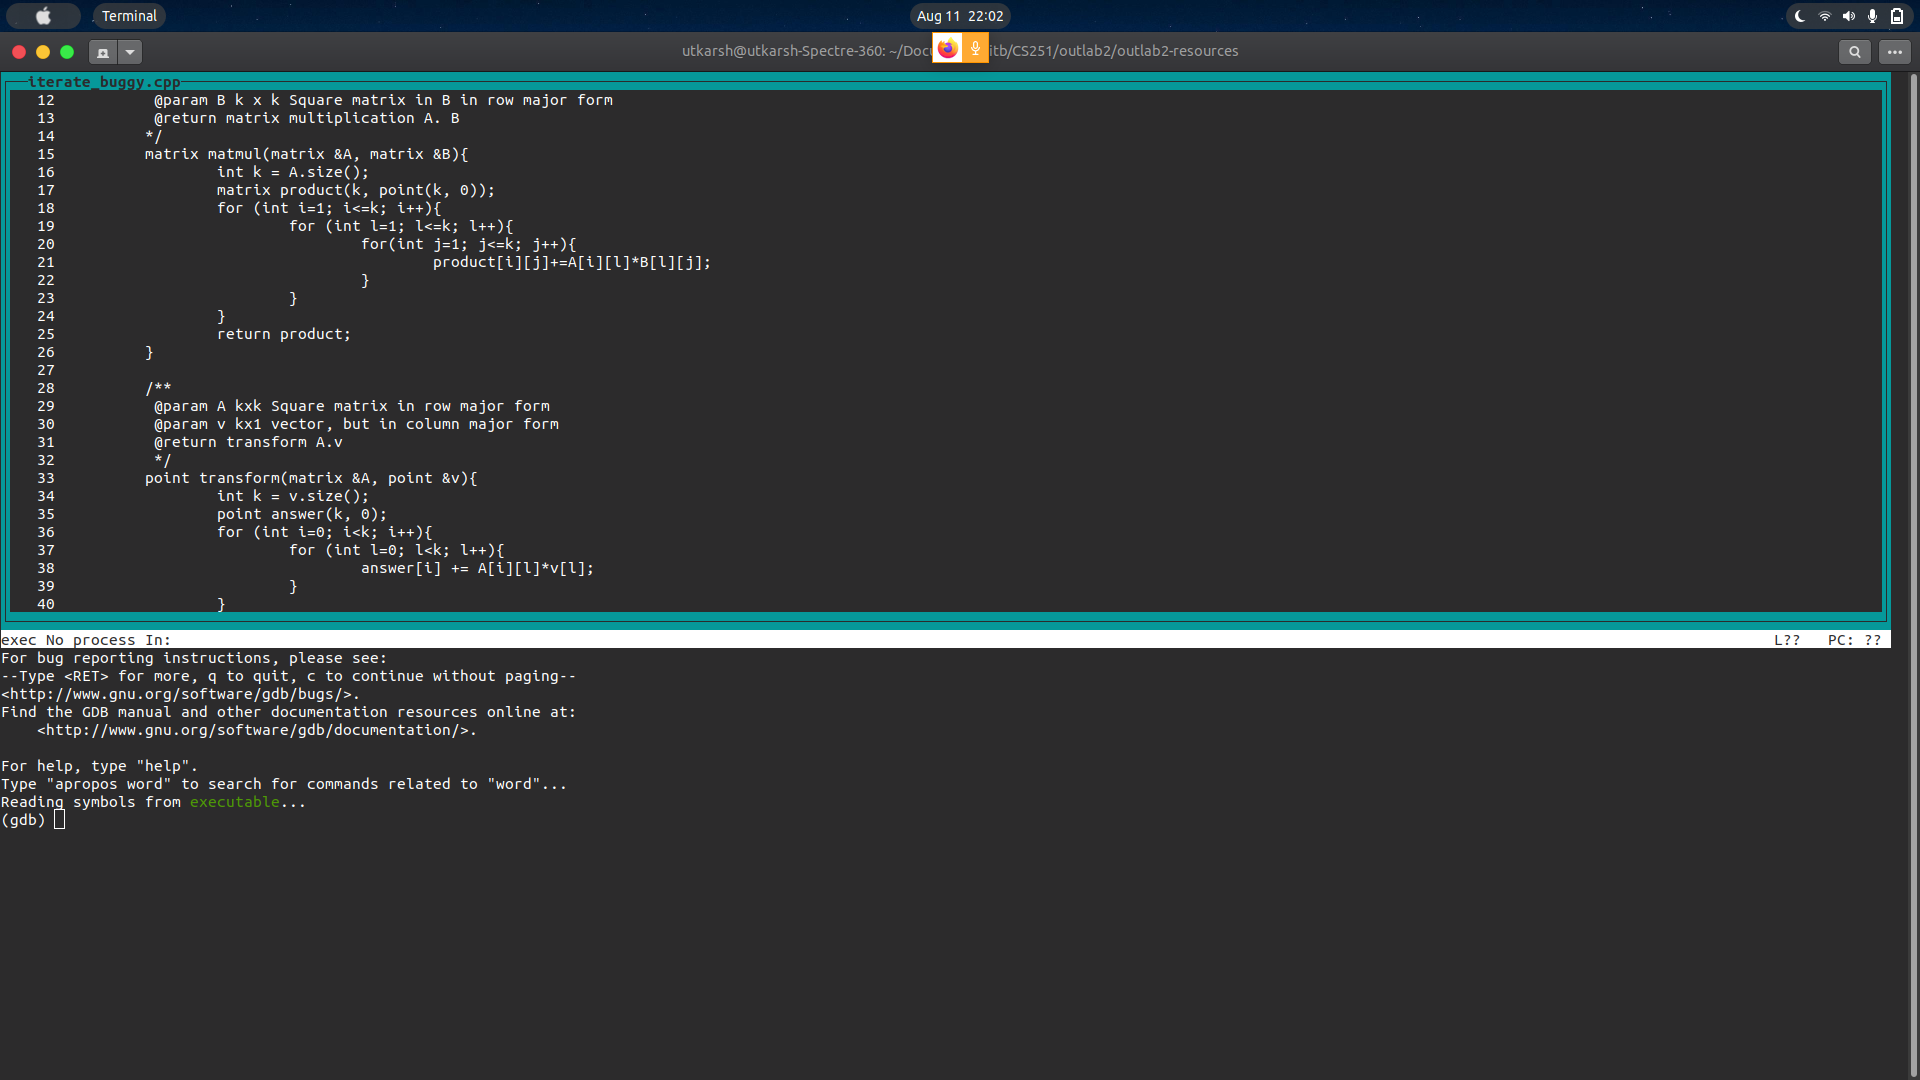
\includegraphics[height=\CommonHeight]{aristotle.png}}
                {\caption{Screenshot when code showed up}}
                \ffigbox[\FBwidth]
                {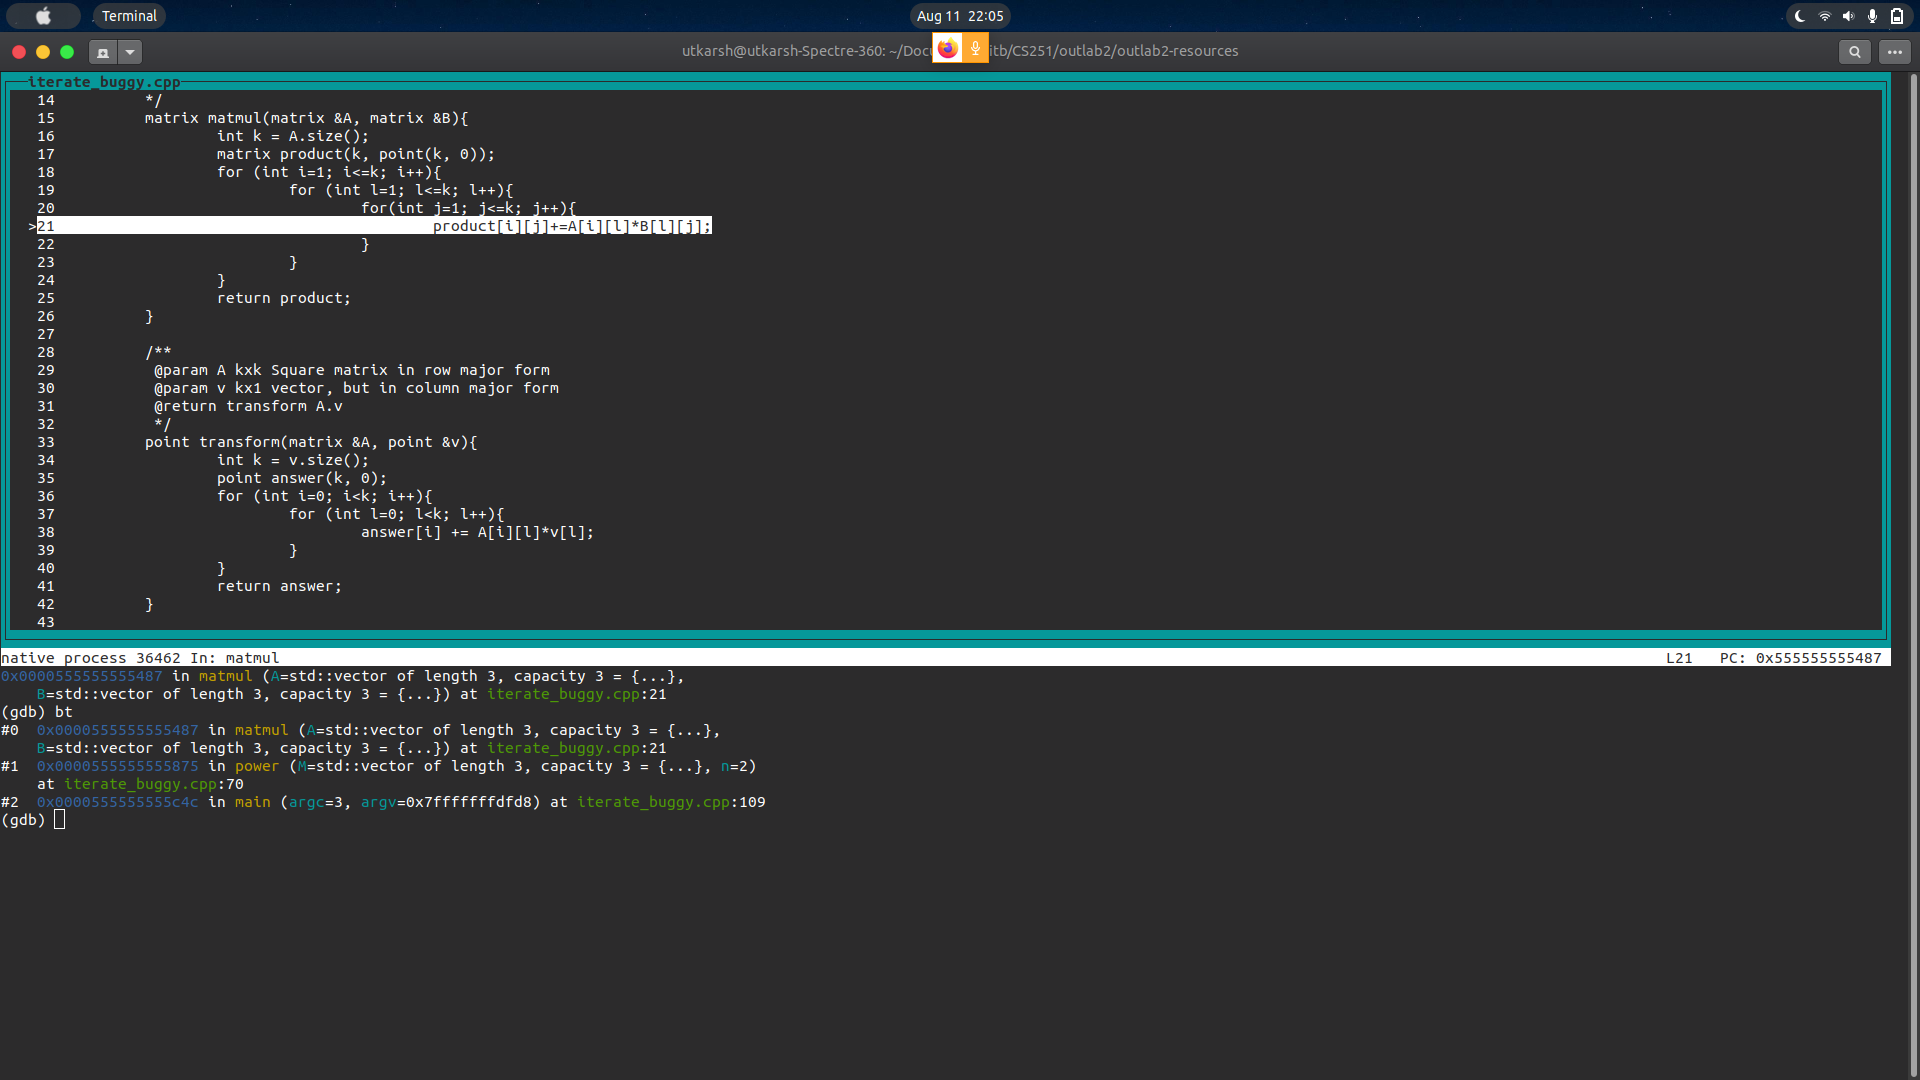
\includegraphics[height=\CommonHeight]{kripke.png}}
                {\caption{Output of (gdb) bt}}
            \end{floatrow}}
\end{figure}

\subsection{gdb outputs}
\$1 = std::vector of length 2, capacity 2 = \{std::vector of length 2, capacity 2 = \{1, 0\},
  std::vector of length 2, capacity 2 = \{0, 1\}\}

\$2 = std::stack wrapping: std::deque with 9 elements = \{1, 1, 1, 1, 1, 1, 0, 1, 1\}

\subsection{Table}
\begin{center}
\begin{tabular}{ l | c | c } 
    \hline
    \textbf{operations} & \textbf{working} \\ 
    \hline
    \{1,1,1,1,1,1,0,1,1\} & \{1,0,0,1\} \\ 
    \hline
    \{1,1,1,1,1,1,0,1\} & \{1,0,1,1\} \\
    \hline
    \{1,1,1,1,1,1,0\} & \{1,2,2,3\} \\
    \hline
    \{1,1,1,1,1,1\} & \{5,8,8,3\} \\
    \hline
    \{1,1,1,1,1\} & \{144,233,233,377\} \\
    \hline
    \{1,1,1,1\} & \{121393,196418,196418,317811\} \\
    \hline
    \{1,1,1\} & \{8e+10,1e+11,1e+11,2e+11\} \\
    \hline
    \{1,1\} & \{8e+14,1e+15,1e+15,2e+15\}\\
    \hline
    \{1\} & \{4e+22,7e+22,7e+22,1e+23\} \\
    \hline
    \{\} & \{1e+46,2e+46,2e+46,3e+46\} \\
    \hline
\end{tabular}
\end{center}

\pagebreak

\section{Hints and tips}

% \begin{code}
% \documentclass{article}
% %...
% \usepackage[linesnumbered,ruled,vlined]{algorithm2e}
% %...
% \begin{document}
% %...
% \begin{algorithm}[ht]
% \caption{...}
% \SetAlgoLined
% \DontPrintSemicolon
% \KwData{...}
% \KwResult{...}
% Statement \;
% %Let magic happen here
% $ a \gets b \cdot \function(c)\%d */ $ \;
% \end{algorithm}
% %...
% \end{document}
% \end{code}

\begin{code}
\documentclass{article}
\usepackage[utf8]{inputenc}
\usepackage[a4paper,hmargin=1.2 in,bottom =1.5 in]{geometry}
\usepackage[parfill]{parskip}
\usepackage{hyperref}
\usepackage{fancyhdr}
\usepackage{enumitem}
\usepackage{amsmath}
\usepackage{amsthm}
\usepackage{amssymb}
\usepackage[linesnumbered,ruled,vlined]{algorithm2e}
\usepackage{listings}
\usepackage{xcolor}
\usepackage{floatrow}
\usepackage{graphicx}
\bibliographystyle{plainurl}
\bibliography{biblio}
\end{code}

This is my Listing \ref{env: listing}

\bibliography{biblio}
\end{document}